\documentclass[10 pt,usenames,dvipsnames, oneside]{article}
\usepackage{../../../modelo-ensino-medio}



\begin{document}

\begin{center}
  \begin{minipage}[l]{3cm}

\includegraphics[width=2cm]{logo}    
\end{minipage}\hfill
\begin{minipage}[r]{.8\textwidth}
 {\Large \scshape Atividade: Comparando funções conhecidas}  
\end{minipage}
\end{center}
\vspace{.2cm}

\ifdefined\prof
%Habilidades da BNCC
\begin{objetivos}
\item \textbf{EM13MAT403} Analisar e estabelecer relações, com ou sem apoio de tecnologias digitais, entre as representações de funções exponencial e logarítmica expressas em tabelas e em plano cartesiano, para identificar as características fundamentais (domínio, imagem, crescimento) de cada função.
\end{objetivos}

%Caixa do Para o Professor
\begin{goals}
%Objetivos específicos
\begin{enumerate}
\item Identificar gráficos de funções logarítmicas em bases e contextos distintos.
\end{enumerate}

\tcblower

%Orientações e sugestões
\begin{itemize}
\item A atividade \textit{"Comparando funções conhecidas"} compara o gráfico da função logarítmica com os gráficos de outras funções conhecidas. Essa comparação ajuda a distinguir a função recém apresentada das demais e serve de preparação para as aplicações práticas a seguir, que demandam o conhecimento do perfil da função.
\end{itemize}
\end{goals}

\bigskip
\begin{center}
{\large \scshape Atividade}
\end{center}
\fi

As curvas na figura a seguir representam as funções $f(x) = 2x-3$, $g(x)=2x^2-1$, $h(x)=1{,}5^x$ e $l(x)=\log_2 x$. Identifique que curva representa cada função. Calcular o valor da função para alguns valores de $x$ pode auxiliar na identificação.

\begin{figure}[H]
\centering

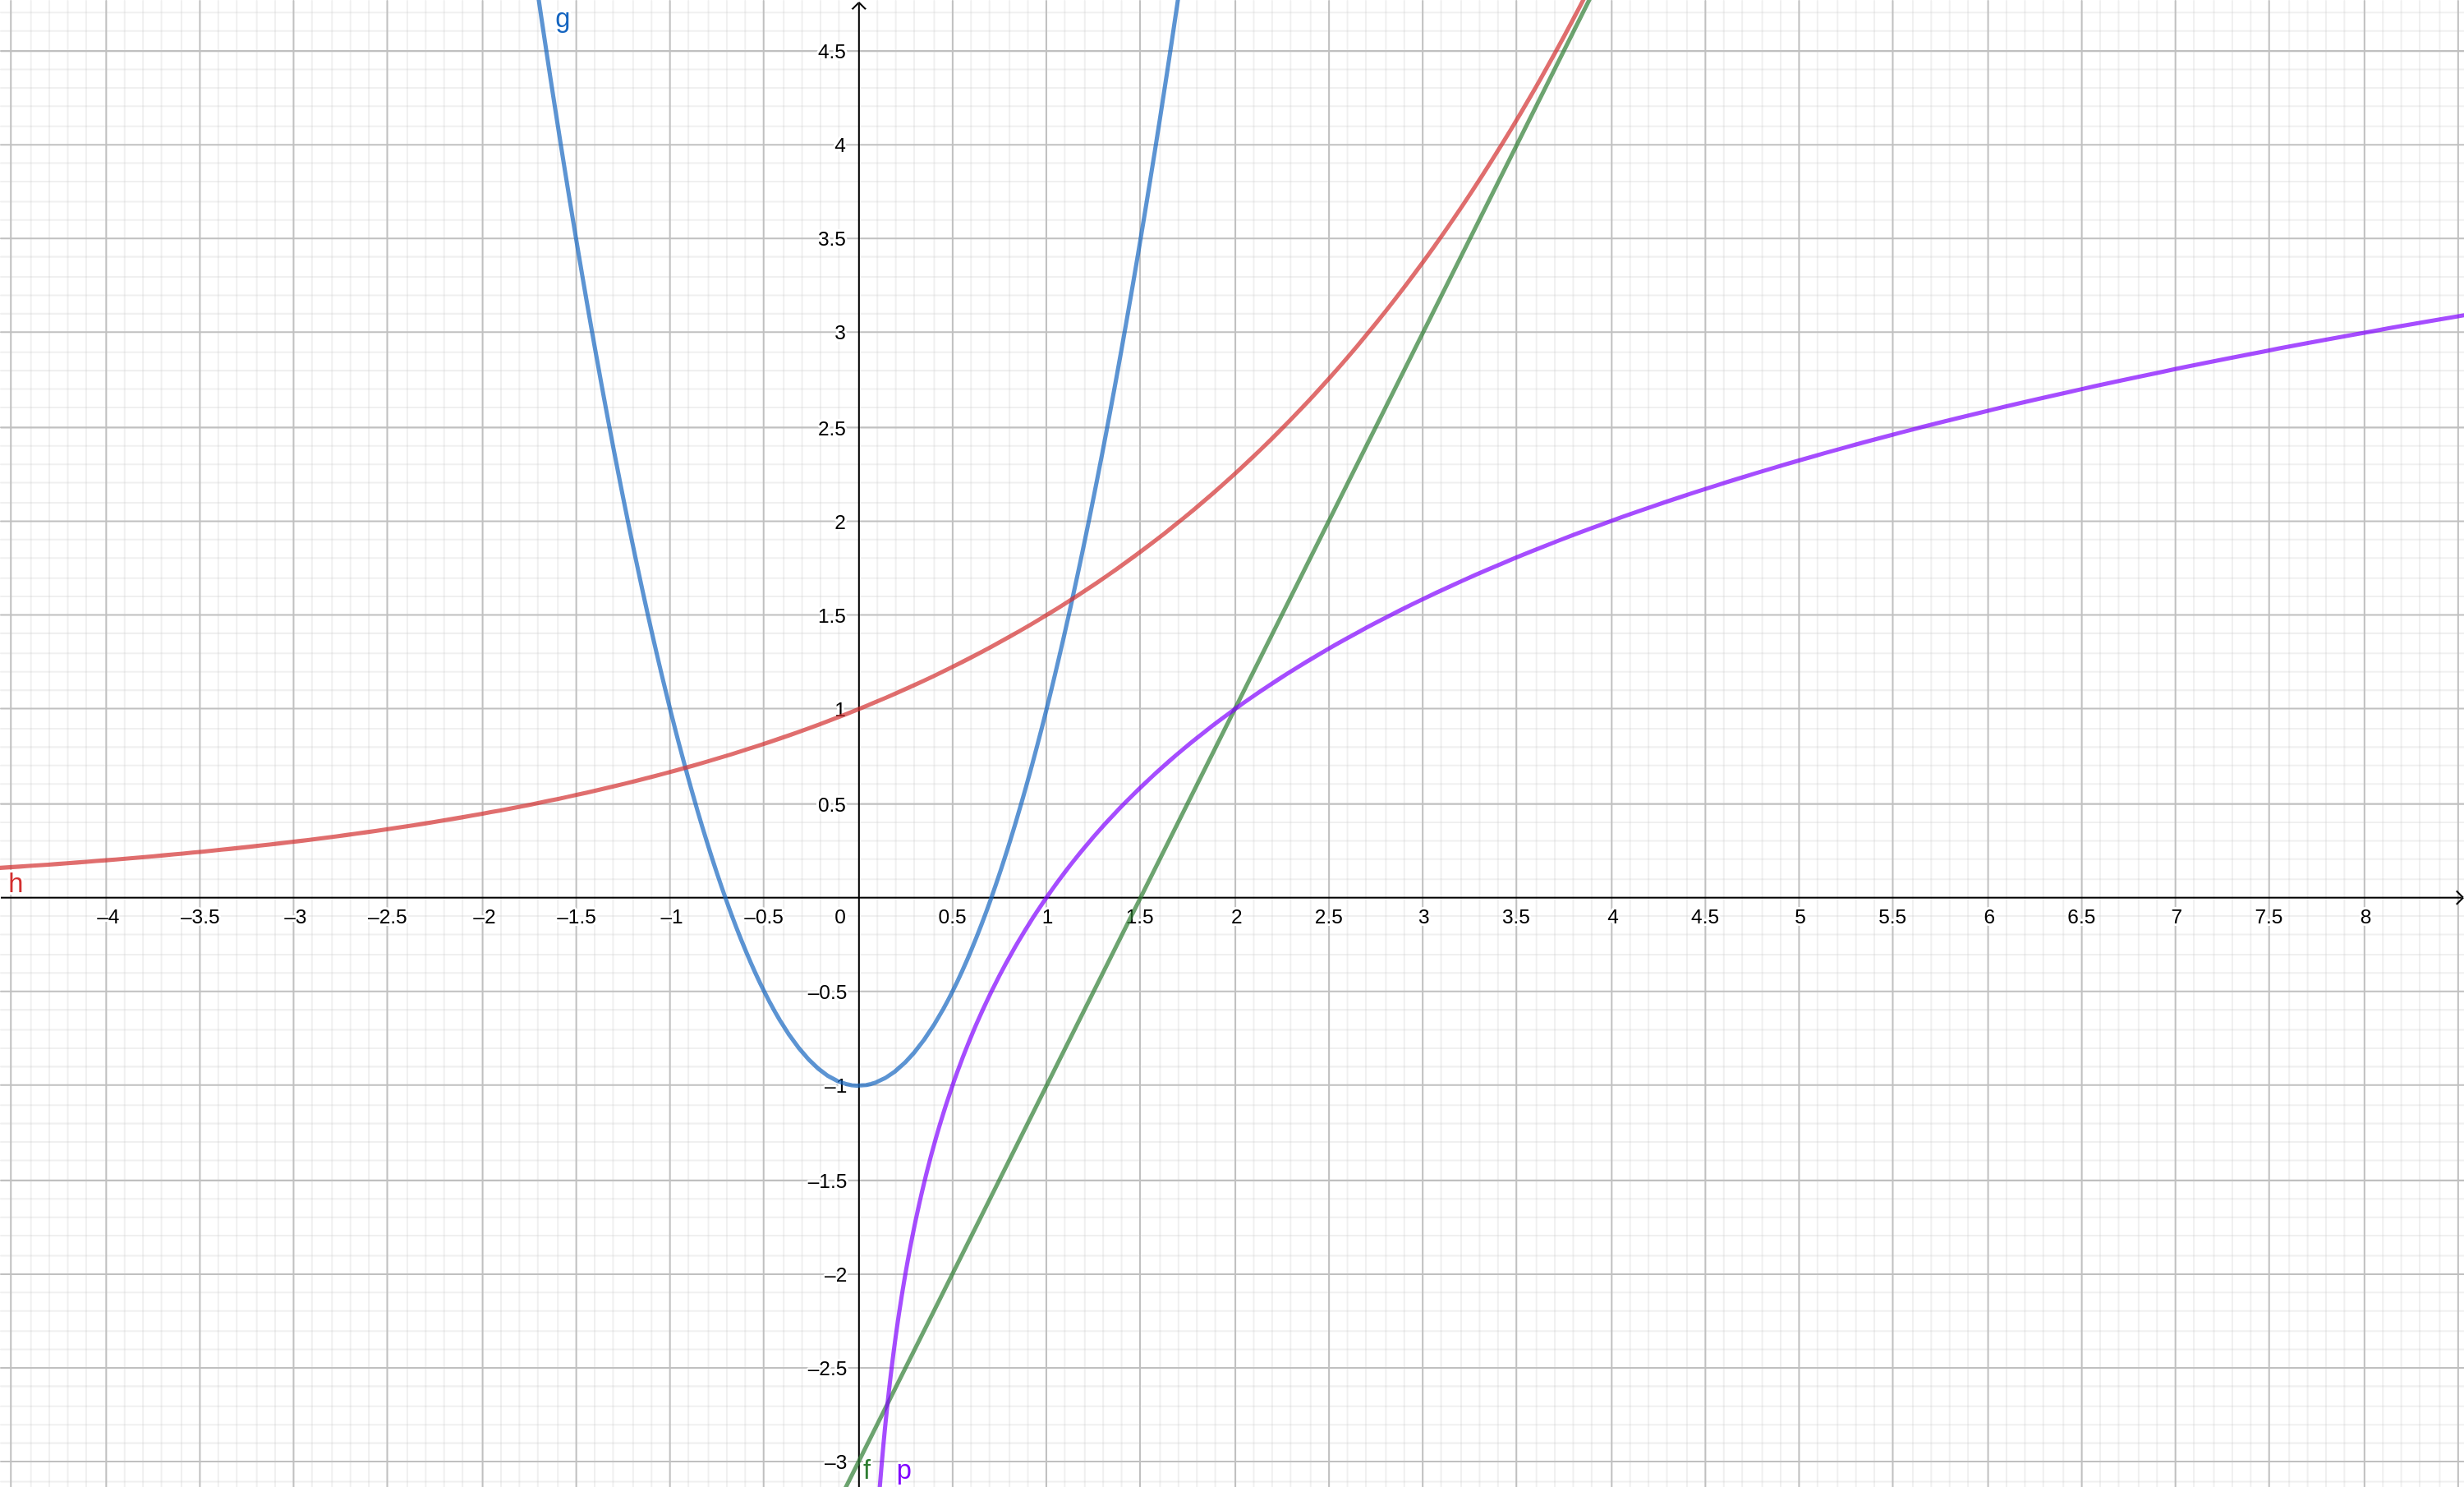
\includegraphics[width=\linewidth]{graficos_varias_funcoes}
\end{figure}

\ifdefined\prof

\begin{solucao}



	$f(x)$ descreve uma reta e foi plotada em verde, $g(x)$ descreve uma parábola e foi plotada em azul, $h(x)$ descreve uma exponencial, cujos valores são sempre positivos, e foi plotada em vermelho e $l(x)$ é uma função logarítmica, definida apenas no semi-eixo positivo, e foi plotada em roxo.
\end{solucao}
\fi

\end{document}